\documentclass{article}
%% %\VignetteIndexEntry{MotifDb Overview}
%% %\VignettePackage{MotifDb}
\usepackage[noae]{Sweave}
\usepackage[left=0.5in,top=0.5in,right=0.5in,bottom=0.75in,nohead,nofoot]{geometry} 
\usepackage{hyperref}
\usepackage[noae]{Sweave}
\usepackage{color}
\usepackage{graphicx}
\usepackage{caption}
\usepackage{subcaption}

\definecolor{Blue}{rgb}{0,0,0.5}
\definecolor{Green}{rgb}{0,0.5,0}

\RecustomVerbatimEnvironment{Sinput}{Verbatim}{%
  xleftmargin=1em,%
  fontsize=\small,%
  fontshape=sl,%
  formatcom=\color{Blue}%
  }
\RecustomVerbatimEnvironment{Soutput}{Verbatim}{%
  xleftmargin=0em,%
  fontsize=\scriptsize,%
  formatcom=\color{Blue}%
  }
\RecustomVerbatimEnvironment{Scode}{Verbatim}{xleftmargin=2em}



\renewenvironment{Schunk}{\vspace{\topsep}}{\vspace{\topsep}}
\fvset{listparameters={\setlength{\topsep}{6pt}}}
% These determine the rules used to place floating objects like figures 
% They are only guides, but read the manual to see the effect of each.
\renewcommand{\topfraction}{.99}
\renewcommand{\bottomfraction}{.99}
\renewcommand{\textfraction}{0.0}

\title{MotifDb} 
\author{Paul Shannon}

\begin{document} 

\maketitle
\begin{abstract}
Many kinds of biological activity are regulated by the binding of proteins to their cognate
substrates.  Of particular interest is the sequence-specific binding of transcription factors to DNA, often in
regulatory regions just upstream of the transcription start site of a gene.  These binding events play a pivotal
role in regulating gene expression.  Sequence specificity among closely related binding sites is nearly always incomplete: some variety
in the DNA sequence is routinely observed.  For this reason, these inexact binding sequence patterns are commonly
described as \emph{motifs} represented numerically as frequency matrices, and visualized as sequence logos.  Despite their importance
in current research, there has been until now no single, annotated, comprehensive collection of publicly available motifs.
The current package provides such a collection, offering more than two thousand annotated matrices from multiple organisms, within the
context of the Bioconductor project.  The matrices can be filtered and selected on the basis of their metadata, used with other
Bioconductor packages (MotIV for motif comparison, seqLogo for visualization) or easily exported for use with 
standard software and websites such as those provided by the MEME Suite\footnote{http://meme.sdsc.edu/meme/doc/meme.html}.
\end{abstract}

\tableofcontents

\section{Introduction and Basic Operations}

The first step is to load the necessary packages:

\begin{Schunk}
\begin{Sinput}
> library (MotifDb)
> library (MotIV)
> library (seqLogo)
\end{Sinput}
\end{Schunk}


%% MotifDb provides two kinds of loosely linked data:  position frequency matrices, and metadata about each matrix.  The matrix
%% names, and the rownames of the metadata table, are identical, so it is easy to map back and forth between
%% the two.  Some measure of convenience is gained by extracting these two kinds of data into separate variables,
%% as we shall see.  The cost in extra memory should not significant.
%% 
%% <<all.matrices>>=
%% matrices.all = as.list (MotifDb)
%% metadata <- values (MotifDb)
%% @ 
There are  more than two thousand  matrices, from five sources:
\begin{Schunk}
\begin{Sinput}
> length (MotifDb)
\end{Sinput}
\begin{Soutput}
[1] 2086
\end{Soutput}
\begin{Sinput}
> sort (table (values (MotifDb)$dataSource), decreasing=TRUE)
\end{Sinput}
\begin{Soutput}
FlyFactorSurvey     JASPAR_CORE            hPDI        UniPROBE          ScerTF 
            614             459             437             380             196 
\end{Soutput}
\end{Schunk}
And 22 organisms (though the majority of the matrices come from just four):
\begin{Schunk}
\begin{Sinput}
> sort (table (values (MotifDb)$organism), decreasing=TRUE)
\end{Sinput}
\begin{Soutput}
Dmelanogaster      Hsapiens   Scerevisiae     Mmusculus   Rnorvegicus 
          739           505           464           329             8 
     Celegans         Zmays     Athaliana    Vertebrata        Amajus 
            7             6             5             4             3 
     Psativum        Gallus   Pfalciparum       Cparvum      Hroretzi 
            3             2             2             1             1 
     Hvulgare   Nsylvestris    Ocuniculus      Phybrida       Rrattus 
            1             1             1             1             1 
    Taestivam       Xlaevis 
            1             1 
\end{Soutput}
\end{Schunk}

With these categories of metadata
\begin{Schunk}
\begin{Sinput}
> colnames (values (MotifDb))
\end{Sinput}
\begin{Soutput}
 [1] "providerName"    "providerId"      "dataSource"      "geneSymbol"     
 [5] "geneId"          "geneIdType"      "proteinId"       "proteinIdType"  
 [9] "organism"        "sequenceCount"   "bindingSequence" "bindingDomain"  
[13] "tfFamily"        "experimentType"  "pubmedID"       
\end{Soutput}
\end{Schunk}
\section{Selection}

There are three ways to extract subsets of interest from the MotifDb collection.  All three operate upon the MotifDb metadata,
matching values in one or more of those fifteen attributes (listed just above), and returning the subset of MotifDb  which 
meet the specified criteria.  The three techniques:  \emph{query}, \emph{subset} and \emph{grep}

\subsection{query}
This is the simplest technique to use, and will suffice in many circumstances.  For example, if you want 
all of the human matrices:
\begin{Schunk}
\begin{Sinput}
> query (MotifDb, 'hsapiens')
\end{Sinput}
\begin{Soutput}
MotifDb object of length 505
| Created from downloaded public sources: 2012-Jul6
| 505 position frequency matrices from 3 sources:
|        JASPAR_CORE:   66
|           UniPROBE:    2
|               hPDI:  437
| 1 organism/s
|           Hsapiens:  505
Hsapiens-hPDI-ABCF2 
Hsapiens-hPDI-ACF 
Hsapiens-hPDI-ACO1 
Hsapiens-hPDI-ADARB1 
Hsapiens-hPDI-AFF4 
...
Hsapiens-JASPAR_CORE-SP1-MA0079.2 
Hsapiens-JASPAR_CORE-ESR2-MA0258.1 
Hsapiens-JASPAR_CORE-HIF1A::ARNT-MA0259.1 
Hsapiens-UniPROBE-Sox4.UP00401 
Hsapiens-UniPROBE-Oct_1.UP00399 
\end{Soutput}
\end{Schunk}
If you want all matrices associated with \textbf{\emph{Sox}} transcription factors, regardless of dataSource or organism:
\begin{Schunk}
\begin{Sinput}
> query (MotifDb, 'sox')
\end{Sinput}
\begin{Soutput}
MotifDb object of length 24
| Created from downloaded public sources: 2012-Jul6
| 24 position frequency matrices from 4 sources:
|    FlyFactorSurvey:    2
|        JASPAR_CORE:    5
|           UniPROBE:   15
|               hPDI:    2
| 3 organism/s
|          Mmusculus:   18
|           Hsapiens:    4
|      Dmelanogaster:    2
Dmelanogaster-FlyFactorSurvey-Sox14_SANGER_10_FBgn0005612 
Dmelanogaster-FlyFactorSurvey-Sox15_SANGER_5_FBgn0005613 
Hsapiens-hPDI-SOX13 
Hsapiens-hPDI-SOX14 
Hsapiens-JASPAR_CORE-SOX9-MA0077.1 
...
Mmusculus-UniPROBE-Sox30.UP00023 
Mmusculus-UniPROBE-Sox4.UP00062 
Mmusculus-UniPROBE-Sox5.UP00091 
Mmusculus-UniPROBE-Sox7.UP00034 
Mmusculus-UniPROBE-Sox8.UP00051 
\end{Soutput}
\end{Schunk}
For all yeast transcription factors with a homeo domain
\begin{Schunk}
\begin{Sinput}
> query (query (MotifDb, 'cerevisiae'), 'homeo')
\end{Sinput}
\begin{Soutput}
MotifDb object of length 14
| Created from downloaded public sources: 2012-Jul6
| 14 position frequency matrices from 2 sources:
|        JASPAR_CORE:   10
|           UniPROBE:    4
| 1 organism/s
|        Scerevisiae:   14
Scerevisiae-UniPROBE-Cup9.UP00308 
Scerevisiae-UniPROBE-Matalpha2.UP00307 
Scerevisiae-UniPROBE-Pho2.UP00268 
Scerevisiae-UniPROBE-Yox1.UP00274 
Scerevisiae-JASPAR_CORE-CUP9-MA0288.1 
...
Scerevisiae-JASPAR_CORE-STE12-MA0393.1 
Scerevisiae-JASPAR_CORE-TEC1-MA0406.1 
Scerevisiae-JASPAR_CORE-TOS8-MA0408.1 
Scerevisiae-JASPAR_CORE-YHP1-MA0426.1 
Scerevisiae-JASPAR_CORE-YOX1-MA0433.1 
\end{Soutput}
\end{Schunk}
The last example may inspire more confidence in the precision of the result than is justified, and for a couple
of reasons.  First, the assignment of  protein binding domains to specific categories is, as of 2012, an ad hoc 
and incomplete process.  Second, the query commands matches the supplied character string to \emph{all} metadata
columns.  In this case, 'homeo' appears both in the \emph{bindingDomain} column and the \emph{tfFamily} column,
and the above \emph{query} will return matches from both.
Searching and filtering should always be accompanined by close scrutiny of the data, such as these commands
illustrate:

\begin{Schunk}
\begin{Sinput}
> unique (grep ('homeo', values(MotifDb)$bindingDomain, ignore.case=T, v=T))
\end{Sinput}
\begin{Soutput}
 [1] "Homeobox"                          "Hox9_act;Homeobox"                
 [3] "LIM;Homeobox"                      "PAX;Homeobox"                     
 [5] "OAR;Homeobox"                      "Pou;Homeobox"                     
 [7] "Distant similarity to homeodomain" "Homeo"                            
 [9] "Homeo, PAX"                        "Homeo, POU"                       
\end{Soutput}
\begin{Sinput}
> unique (grep ('homeo', values(MotifDb)$tfFamily, ignore.case=T, v=T))
\end{Sinput}
\begin{Soutput}
[1] "Homeo"                                
[2] "Homeo::Nuclear Factor I-CCAAT-binding"
\end{Soutput}
\end{Schunk}
\subsection{grep}
This selection method (and the next, \emph{subset}) require that you address metadata columns explicitly.  This is a little more
work, but the requisite direct engagement with the metadata is worthwhile.  Repeating the 'query' examples from above,
you can see how more knowedge of MotifDb metadata is required.
\begin{Schunk}
\begin{Sinput}
> mdb.human <- MotifDb [grep ('Hsapiens', values (MotifDb)$organism)]
> mdb.sox <- MotifDb [grep ('sox', values (MotifDb)$geneSymbol, ignore.case=TRUE)]
> yeast.indices = grepl ('scere', values (MotifDb)$organism, ignore.case=TRUE)
> homeo.indices.domain = grepl ('homeo', values (MotifDb)$bindingDomain, ignore.case=TRUE)
> homeo.indices.family = grepl ('homeo', values (MotifDb)$tfFamily, ignore.case=TRUE)
> yeast.homeo.indices = yeast.indices & (homeo.indices.domain | homeo.indices.family)
> yeast.homeoDb = MotifDb [yeast.homeo.indices]
\end{Sinput}
\end{Schunk}

An alternate and somewhat more compact approach:
\begin{Schunk}
\begin{Sinput}
> yeast.homeo.indices <- with(values(MotifDb),
+   grepl('scere', organism, ignore.case=TRUE) &
+     (grepl('homeo', bindingDomain, ignore.case=TRUE) |
+      grepl('homeo', tfFamily, ignore.case=TRUE)))
> 
\end{Sinput}
\end{Schunk}
\subsection{subset}
MotifDb::subset emulates the R base data.frame \emph{subset} command, which is not unlike an SQL select function.
Unfortunately -- and just like the R base subset function -- this MotifDb method cannot be used reliably  within a script:
\emph{It is only reliable when called interactively.}  Here, with mixed success (as you will see) , we use MotifDb::subset to
reproduce the \emph{query} and \emph{grep} selections shown above.

\begin{Schunk}
\begin{Sinput}
> if (interactive ())
+   subset (MotifDb, organism=='Hsapiens')
\end{Sinput}
\end{Schunk}
One can easily find all the 'sox' genes with the subset command, avoiding possible upper/lower case conflicts by passing
the metadata's geneSymbol column through the function 'tolower':
\begin{Schunk}
\begin{Sinput}
> if (interactive ())
+   subset (MotifDb, tolower (geneSymbol) == 'sox4')
\end{Sinput}
\end{Schunk}
Similarly, subset has limited application for a permissive 'homeo' search.
But for the retrieval by explicitly specified search terms, subset works very well:
\begin{Schunk}
\begin{Sinput}
> if (interactive ())
+   subset (MotifDb, organism=='Scerevisiae' & bindingDomain=='Homeo')
\end{Sinput}
\end{Schunk}

\subsection{The Egr1 Case Study}

We now do a simple geneSymbol search, followed by an examination of the sub-MotifDb the search returns.  We are looking for all matrices
associated with the well-known and highly conserved zinc-finger transcription factor, Egr1.
There are two of these in MotifDb, both from mouse, and each from a different data source.

\begin{Schunk}
\begin{Sinput}
>   # subset is convenient: 
> if (interactive ())
+   as.list (subset (MotifDb, tolower (geneSymbol) == 'egr1'))
>   # grep returns indices which allow for more flexibility
> indices = grep ('egr1', values (MotifDb)$geneSymbol, ignore.case=TRUE)  
> length (indices)
\end{Sinput}
\begin{Soutput}
[1] 2
\end{Soutput}
\end{Schunk}
There are a variety of ways to examine and extract data from this object, a MotifList of length 2.  
\begin{Schunk}
\begin{Sinput}
> MotifDb [indices]
\end{Sinput}
\begin{Soutput}
MotifDb object of length 2
| Created from downloaded public sources: 2012-Jul6
| 2 position frequency matrices from 2 sources:
|        JASPAR_CORE:    1
|           UniPROBE:    1
| 1 organism/s
|          Mmusculus:    2
Mmusculus-JASPAR_CORE-Egr1-MA0162.1 
Mmusculus-UniPROBE-Egr1.UP00007 
\end{Soutput}
\end{Schunk}

Now view the matrices as a named list:
\begin{Schunk}
\begin{Sinput}
> as.list (MotifDb [indices])
\end{Sinput}
\begin{Soutput}
$`Mmusculus-JASPAR_CORE-Egr1-MA0162.1`
           1          2         3 4   5   6          7 8         9 10
A 0.20000000 0.13333333 0.0000000 0 0.0 0.2 0.06666667 0 0.1333333  0
C 0.26666667 0.06666667 0.8666667 0 0.0 0.0 0.00000000 0 0.6666667  0
G 0.06666667 0.80000000 0.0000000 1 0.2 0.8 0.93333333 1 0.0000000  1
T 0.46666667 0.00000000 0.1333333 0 0.8 0.0 0.00000000 0 0.2000000  0
          11
A 0.06666667
C 0.00000000
G 0.46666667
T 0.46666667

$`Mmusculus-UniPROBE-Egr1.UP00007`
          1          2          3          4           5           6
A 0.2115466 0.14198757 0.03260499 0.11512588 0.003516173 0.004715059
C 0.2827083 0.72243721 0.87717185 0.07060553 0.990021152 0.982482238
G 0.2034722 0.05485440 0.01243161 0.78128969 0.002264928 0.009896878
T 0.3022730 0.08072082 0.07779155 0.03297890 0.004197748 0.002905824
            7           8           9         10         11         12
A 0.001626612 0.262351637 0.005889514 0.02289301 0.02303758 0.56763334
C 0.975937323 0.731731673 0.985755764 0.09046006 0.85994854 0.05739392
G 0.001661635 0.002729558 0.002081402 0.64932246 0.03791264 0.16679165
T 0.020774430 0.003187133 0.006273319 0.23732447 0.07910124 0.20818108
         13        14
A 0.1765973 0.1830489
C 0.3312648 0.1837744
G 0.1253083 0.2267928
T 0.3668295 0.4063840
\end{Soutput}
\end{Schunk}
and finally, the metadata associated with these two matrices, transposed, for easy reading and comparison:
\begin{Schunk}
\begin{Sinput}
> noquote (t (as.data.frame (values (MotifDb [indices]))))
\end{Sinput}
\begin{Soutput}
                Mmusculus-JASPAR_CORE-Egr1-MA0162.1
providerName    Egr1                               
providerId      MA0162.1                           
dataSource      JASPAR_CORE                        
geneSymbol      Egr1                               
geneId          13653                              
geneIdType      ENTREZ                             
proteinId       P08046                             
proteinIdType   UNIPROT                            
organism        Mmusculus                          
sequenceCount   15                                 
bindingSequence <NA>                               
bindingDomain   Zinc-coordinating                  
tfFamily        BetaBetaAlpha-zinc finger          
experimentType  bacterial 1-hybrid                 
pubmedID        16041365                           
                Mmusculus-UniPROBE-Egr1.UP00007
providerName    SCI09/Egr1_pwm_primary.txt     
providerId      UP00007                        
dataSource      UniPROBE                       
geneSymbol      Egr1                           
geneId          13653                          
geneIdType      ENTREZ                         
proteinId       P08046                         
proteinIdType   UNIPROT                        
organism        Mmusculus                      
sequenceCount   <NA>                           
bindingSequence <NA>                           
bindingDomain   ZnF_C2H2                       
tfFamily        <NA>                           
experimentType  protein binding microarray     
pubmedID        19443739                       
\end{Soutput}
\end{Schunk}
 
We used the \emph{grep} function above to find rows in the metadata table whose \emph{geneSymbol} column includes the string 'Egr1'.
If you wish to identify matrices (and/or their attendant metadata) based upon a richer combination of criteria, for instance:

\begin{enumerate}
  \item organism  (\emph{Mmusculus})
  \item gene symbol  (\emph{Egr1})
  \item data source  (\emph{JASPAR\_CORE})
\end{enumerate}

the grep solution, while serviceable, becomes a little awkward:
\begin{Schunk}
\begin{Sinput}
> geneSymbol.rows = grep ('Egr1', values (MotifDb)$geneSymbol, ignore.case=TRUE)
> organism.rows = grep ('Mmusculus', values (MotifDb)$organism, ignore.case=TRUE)
> source.rows = grep ('JASPAR', values (MotifDb)$dataSource, ignore.case=TRUE)
> egr1.mouse.jaspar.rows = intersect (geneSymbol.rows, 
+                            intersect (organism.rows, source.rows))
> print (egr1.mouse.jaspar.rows)
\end{Sinput}
\begin{Soutput}
[1] 1402
\end{Soutput}
\begin{Sinput}
> egr1.motif <- MotifDb [egr1.mouse.jaspar.rows]
\end{Sinput}
\end{Schunk}

Far more concise, and fully reliable as an interactive command (though \emph{not} if used in a 
script\footnote{See the help page of the base R command subset for detail), is the \emph{subset} command}):
\begin{Schunk}
\begin{Sinput}
> if (interactive ()) {
+   egr1.motif <- subset (MotifDb, organism=='Mmusculus' & 
+                         dataSource=='JASPAR_CORE' & 
+                         geneSymbol=='Egr1')
+   }
\end{Sinput}
\end{Schunk}
Whichever method you use, this next chunk of code displays the matrix, and then the metadata for mouse JASPAR Egr1, the latter
textually-transformed for easy reading within the size constraints of this page.
\begin{Schunk}
\begin{Sinput}
> egr1.motif
\end{Sinput}
\begin{Soutput}
MotifDb object of length 1
| Created from downloaded public sources: 2012-Jul6
| 1 position frequency matrices from 1 source:
|        JASPAR_CORE:    1
| 1 organism/s
|          Mmusculus:    1
Mmusculus-JASPAR_CORE-Egr1-MA0162.1 
\end{Soutput}
\begin{Sinput}
> as.list (egr1.motif)
\end{Sinput}
\begin{Soutput}
$`Mmusculus-JASPAR_CORE-Egr1-MA0162.1`
           1          2         3 4   5   6          7 8         9 10
A 0.20000000 0.13333333 0.0000000 0 0.0 0.2 0.06666667 0 0.1333333  0
C 0.26666667 0.06666667 0.8666667 0 0.0 0.0 0.00000000 0 0.6666667  0
G 0.06666667 0.80000000 0.0000000 1 0.2 0.8 0.93333333 1 0.0000000  1
T 0.46666667 0.00000000 0.1333333 0 0.8 0.0 0.00000000 0 0.2000000  0
          11
A 0.06666667
C 0.00000000
G 0.46666667
T 0.46666667
\end{Soutput}
\begin{Sinput}
> noquote (t (as.data.frame (values (egr1.motif))))
\end{Sinput}
\begin{Soutput}
                Mmusculus-JASPAR_CORE-Egr1-MA0162.1
providerName    Egr1                               
providerId      MA0162.1                           
dataSource      JASPAR_CORE                        
geneSymbol      Egr1                               
geneId          13653                              
geneIdType      ENTREZ                             
proteinId       P08046                             
proteinIdType   UNIPROT                            
organism        Mmusculus                          
sequenceCount   15                                 
bindingSequence <NA>                               
bindingDomain   Zinc-coordinating                  
tfFamily        BetaBetaAlpha-zinc finger          
experimentType  bacterial 1-hybrid                 
pubmedID        16041365                           
\end{Soutput}
\end{Schunk}


Next we use the bioconductor \emph{seqLogo} package to display this motif.

\begin{Schunk}
\begin{Sinput}
> seqLogo (as.list (egr1.motif)[[1]])
\end{Sinput}
\end{Schunk}

\begin{figure}[htpb!]
  \centering
  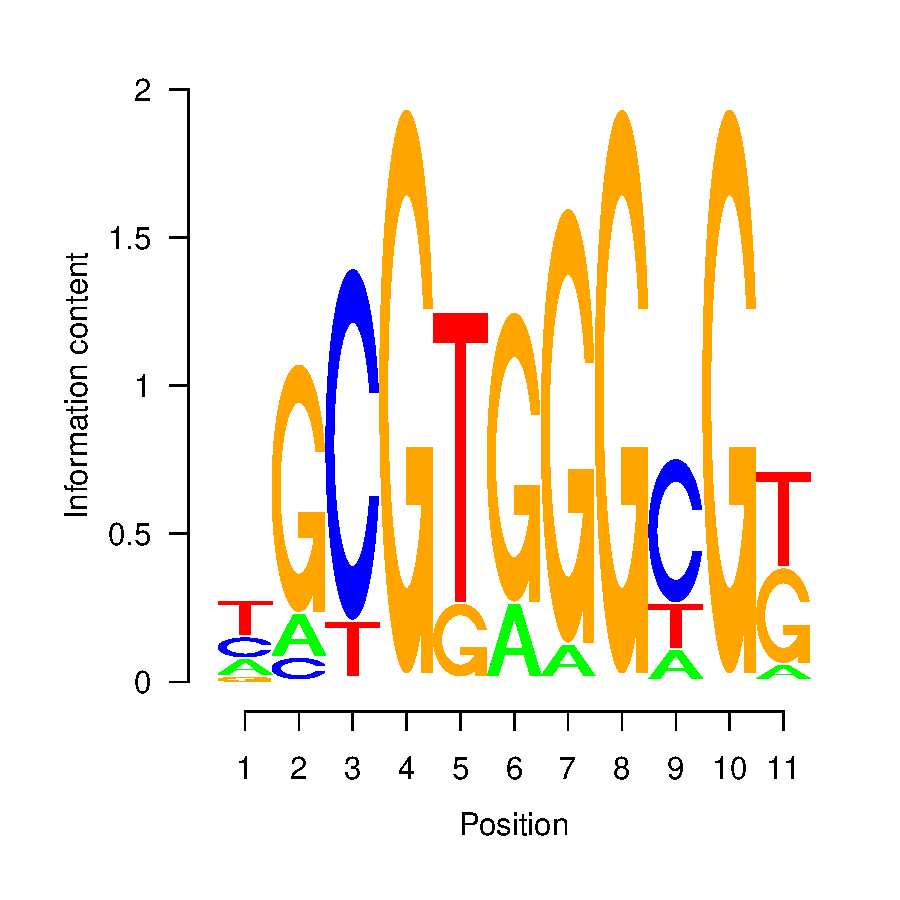
\includegraphics[width=0.3\textwidth]{MotifDb-egr1}
  \caption{Mmusculus-JASPAR\_CORE-Egr1-MA0162.1}
\end{figure}
  
\section{Motif Matching}
We will look for the ten position frequency matrices which are the best match to JASPAR's mouse EGR1, using
the MotIV package.  We actually request the top eleven hits from the entire MotifDb, since the first hit 
should be the target matrix itself, since that is of necessity found in the full MotifDb.

\begin{Schunk}
\begin{Sinput}
> egr1.hits <- motifMatch (as.list (egr1.motif) [1], as.list (MotifDb), top=11)
\end{Sinput}
\begin{Soutput}
	Ungapped Alignment
	Scores read
	Database read
	Motif matches : 11
\end{Soutput}
\begin{Sinput}
> # 'MotIV.toTable' -- defined above (and hidden) -- will become part of MotIV in the upcoming release
> tbl.hits <- MotIV.toTable (egr1.hits)
> print (tbl.hits)
\end{Sinput}
\begin{Soutput}
                                                               name
1                               Mmusculus-JASPAR_CORE-Egr1-MA0162.1
2             Dmelanogaster-FlyFactorSurvey-sr_SANGER_5_FBgn0003499
3                                 Mmusculus-UniPROBE-Zif268.UP00400
4           Dmelanogaster-FlyFactorSurvey-klu_SANGER_10_FBgn0013469
5                                   Mmusculus-UniPROBE-Egr1.UP00007
6            Dmelanogaster-FlyFactorSurvey-klu_SOLEXA_5_FBgn0013469
7            Dmelanogaster-FlyFactorSurvey-Sp1_SANGER_5_FBgn0020378
8        Dmelanogaster-FlyFactorSurvey-Bteb2_SANGER_2.5_FBgn0025679
9  Dmelanogaster-FlyFactorSurvey-CG3065_F1.3_SANGER_2.5_FBgn0034946
10                                 Scerevisiae-ScerTF-SUT1-harbison
11         Dmelanogaster-FlyFactorSurvey-Sp1_SOLEXA_2.5_FBgn0020378
           eVal                sequence                   match strand
1  1.110223e-16             NGCGTGGGCGK             NGCGTGGGCGK      +
2  2.638001e-12          -NGCGTGGGCGK--          NKRNGKGGGCGKNN      +
3  1.550782e-11 ------NGCGTGGGCGK------ NNNNNNTGCGTGGGCGNNNNNTN      -
4  2.341696e-10             NGCGTGGGCGK             TGYGTGGGTGK      +
5  8.184576e-10          --NGCGTGGGCGK-          NNNGCGGGGGCGGN      -
6  1.812032e-08         NGCGTGGGCGK----         NGYGTGGGTGKNNNN      +
7  1.998650e-08          NGCGTGGGCGK---          ---GKGGGCGKRNN      +
8  1.632763e-07             NGCGTGGGCGK             ---GGGGGCGT      +
9  2.892135e-07          NGCGTGGGCGK---          ---GKGGGCGTGGC      +
10 6.714194e-07             NGCGTGGGCGK             -GCSGSGNNSG      +
11 1.033784e-06         NGCGTGGGCGK----         -NNGKGGGCGKRNCN      +
\end{Soutput}
\end{Schunk}

The \emph{sequence} column in this table is the \emph{consensus sequence} -- with heterogeneity left out -- for the 
matrix it describes.   

\vspace{10 mm}

\textbf{\emph{Puzzling: the strand of the match reported above is opposite of what I expected, and opposite of what seqLogo displays.
  This is a question for the MotIV developers.}}

\vspace{10 mm}

The six logos appear below, beginning with the logo of the query matrix, \emph{Mmusculus-JASPAR\_CORE-Egr1-MA0162.1}, including
two other mouse matrices, and two zinc-finger fly matrices.  Examining the three mouse matrices and their metadata reveals that
all three (geneSymbol differences aside) describe the same protein:
\begin{Schunk}
\begin{Sinput}
> if (interactive ())
+   noquote (t (as.data.frame (subset (values (MotifDb), geneId=='13653'))))
\end{Sinput}
\end{Schunk}
Zinc finger protein domains are classified into many \emph{fold groups}; their respective cognate DNA sequence may classify similarly.
That two fly matrices significantly match three reports of the mouse Egr1 motif suggests impressive conservation of this 
binding pattern, or convergent evolution.  

Let us look at the metadata for the first fly match, whose geneId is \textbf{FBgn0003499}:
\begin{Schunk}
\begin{Sinput}
> noquote (t (as.data.frame (values (MotifDb)[grep ('FBgn0003499', values (MotifDb)$geneId),])))
\end{Sinput}
\begin{Soutput}
                Dmelanogaster-FlyFactorSurvey-sr_SANGER_5_FBgn0003499
providerName    sr_SANGER_5_FBgn0003499                              
providerId      FBgn0003499                                          
dataSource      FlyFactorSurvey                                      
geneSymbol      Sr                                                   
geneId          FBgn0003499                                          
geneIdType      FLYBASE                                              
proteinId       E1JIP0                                               
proteinIdType   UNIPROT                                              
organism        Dmelanogaster                                        
sequenceCount     18                                                 
bindingSequence <NA>                                                 
bindingDomain   zf-C2H2                                              
tfFamily        <NA>                                                 
experimentType  bacterial 1-hybrid, SANGER sequencing                
pubmedID        <NA>                                                 
                Dmelanogaster-FlyFactorSurvey-sr_SOLEXA_5_FBgn0003499
providerName    sr_SOLEXA_5_FBgn0003499                              
providerId      FBgn0003499                                          
dataSource      FlyFactorSurvey                                      
geneSymbol      Sr                                                   
geneId          FBgn0003499                                          
geneIdType      FLYBASE                                              
proteinId       E1JIP0                                               
proteinIdType   UNIPROT                                              
organism        Dmelanogaster                                        
sequenceCount   2316                                                 
bindingSequence <NA>                                                 
bindingDomain   zf-C2H2                                              
tfFamily        <NA>                                                 
experimentType  bacterial 1-hybrid, SOLEXA sequencing                
pubmedID        <NA>                                                 
\end{Soutput}
\end{Schunk}
that the SOLEXA motif, based upon 2316 sequences, did not (in work not shown, it appears 22nd in the an expanded
motifMatch hit list, with a eval of 10e-5).  It is possible that the SOLEXA motif is more accurate, and that a close
examination of this case, including sequence logos, position frequency matrices, and the search parameters of
motifMatch, will be instructive.  Repeating the search with \emph{tomtom} might also be illuminating -- either as
confirmation of MotIV and the default parameterization we used, or as a correction to it.  Here we see the facilities
for exploratory data analysis MotifDb provides, and the opportunities for data analysis which result.








\begin{figure}[htpb!]
  \centering
  \begin{subfigure}[b]{0.38\textwidth}
    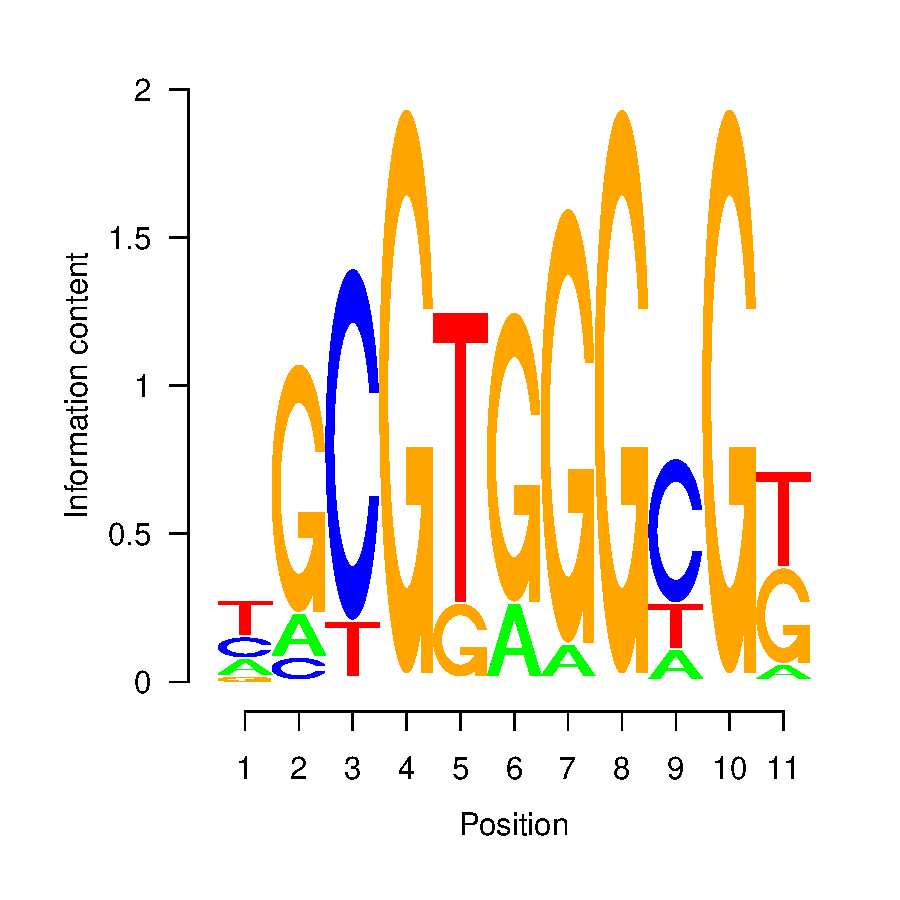
\includegraphics[width=\textwidth]{MotifDb-logo1}
    \caption{Mmusculus-JASPAR\_CORE-Egr1-MA0162.1}
    \label{fig:Egr1-MA0162.1}
    \end{subfigure}%
  \begin{subfigure}[b]{0.38\textwidth}
    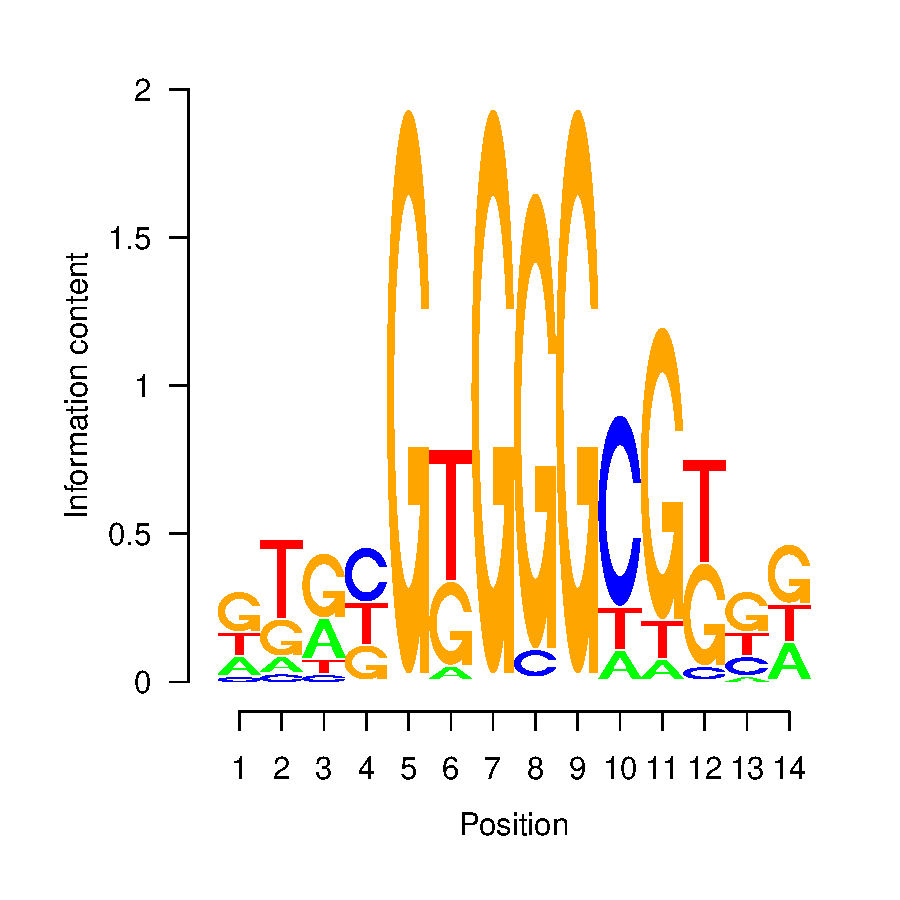
\includegraphics[width=\textwidth]{MotifDb-logo2}
    \caption{Dme-FFS-sr\_SANGER\_5\_FBgn0003499\\(abbreviated)}
    \label{fig:Egr1-logo2}
    \end{subfigure}%
\end{figure}

\begin{figure}[htpb!]
  \centering
  \begin{subfigure}[b]{0.38\textwidth}
    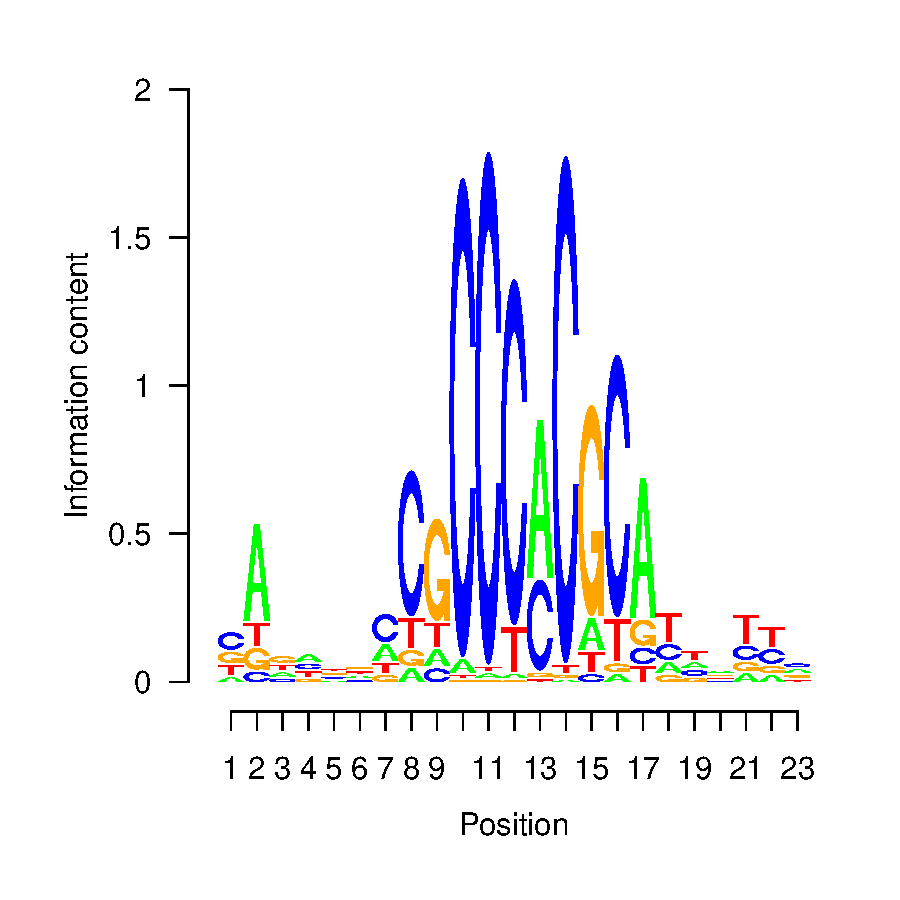
\includegraphics[width=\textwidth]{MotifDb-logo3}
    \caption{Mmusculus-UniPROBE-Zif268.UP00400}
    \label{fig:Egr1-logo3}
    \end{subfigure}%
  \begin{subfigure}[b]{0.38\textwidth}
    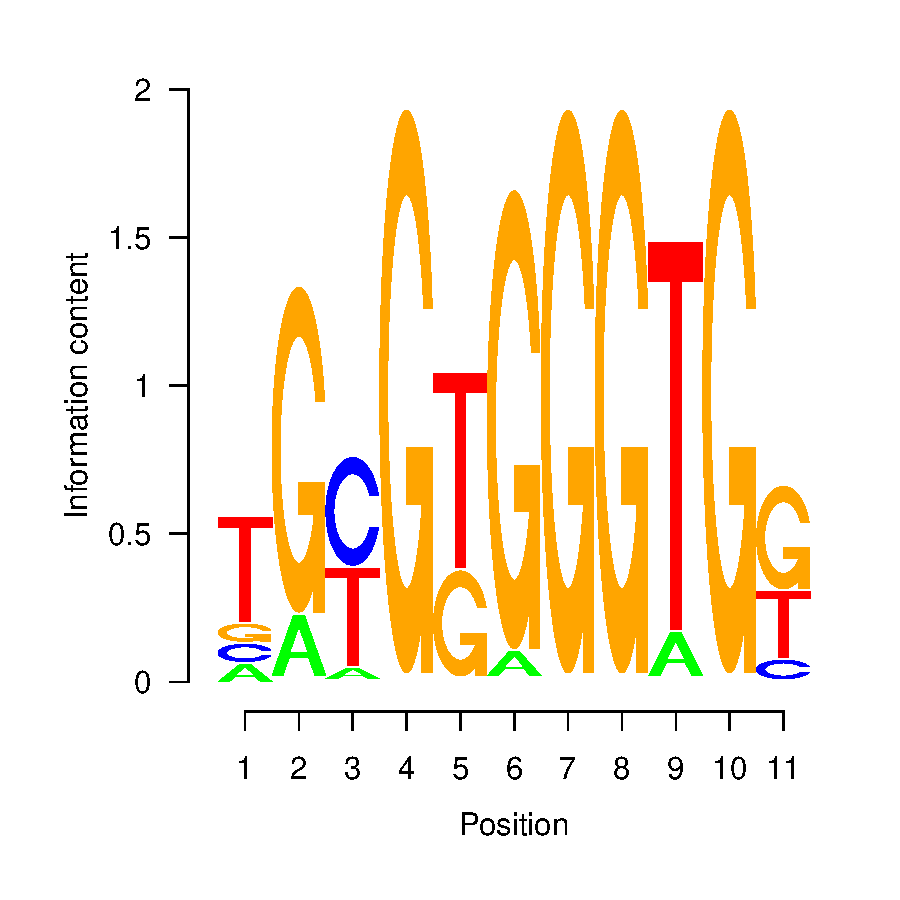
\includegraphics[width=\textwidth]{MotifDb-logo4}
    \caption{Dme-FFS-klu\_SANGER\_10\_FBgn0013469}
    \label{fig:Egr1-logo4}
    \end{subfigure}%
\end{figure}


\begin{figure}[htpb!]
  \centering
  \begin{subfigure}[b]{0.38\textwidth}
    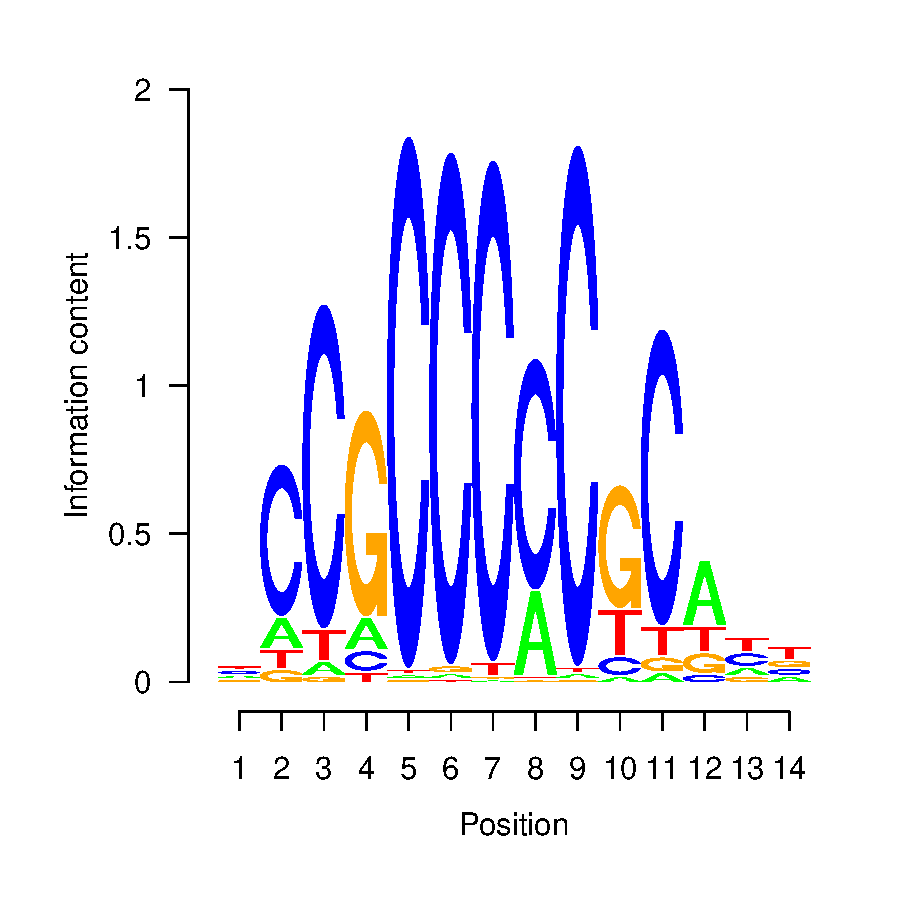
\includegraphics[width=\textwidth]{MotifDb-logo5}
    \caption{Mmusculus-UniPROBE-Egr1.UP00007}
    \label{fig:Egr1-logo5}
    \end{subfigure}%
  \begin{subfigure}[b]{0.38\textwidth}
    \centering
    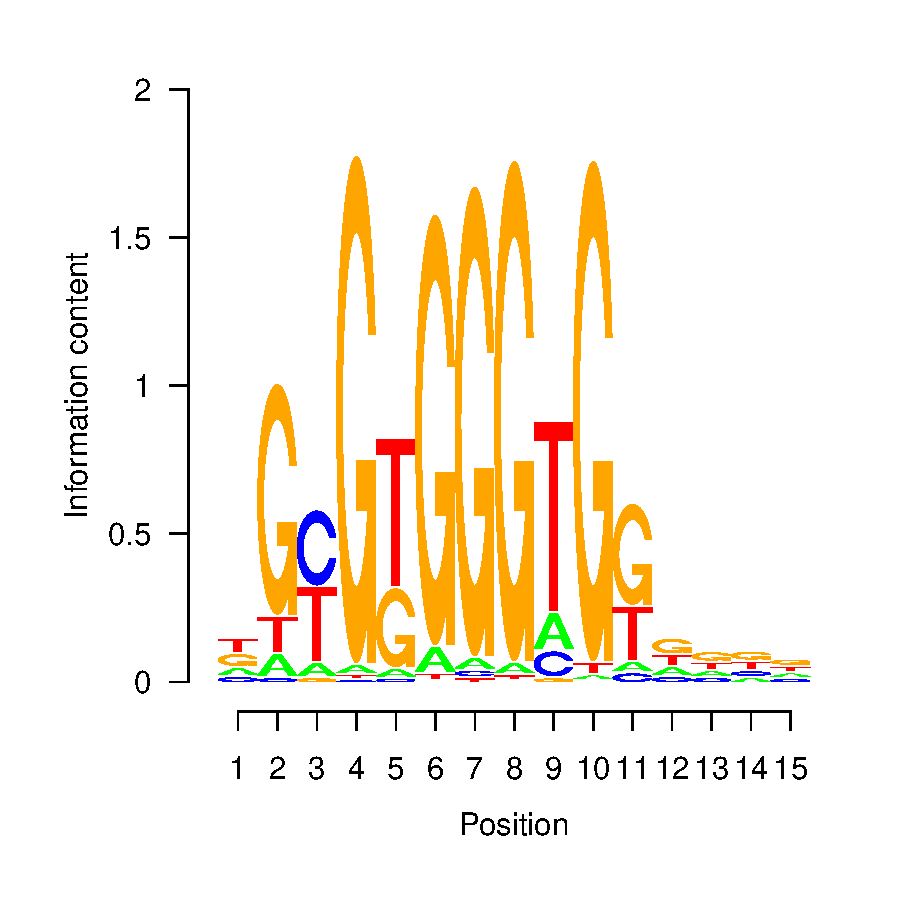
\includegraphics[width=\textwidth]{MotifDb-logo6}
    \caption{Dme-FFS-klu\_SOLEXA\_5\_FBgn0013469}
    \label{fig:Egr1-logo6}
    \end{subfigure}%
\end{figure}

\newpage

\section{Exporting to the MEME Suite}
Some users of this package may wish to export the data -- both matrices and metadata -- so that they may be used in
other programs.  The MEME suite, among others, is broadly useful, continuously improved and well-regarded throughout the
bioinformatics community.  The code below exports all of the MotifDb matrices as a text file in the MEME format, and all
of the metadata as a tab-delimited text file.

\begin{Schunk}
\begin{Sinput}
> matrix.output.file = tempfile ()   # substitute your preferred filename here
> meme.text = export (MotifDb, matrix.output.file, 'meme')
> metadata.output.file = tempfile () # substitute your preferred filename here
> write.table (as.data.frame (values (MotifDb)), file=metadata.output.file, sep='\t', 
+              row.names=TRUE, col.names=TRUE, quote=FALSE)
\end{Sinput}
\end{Schunk}

\section{Future Work}
This first version of MotifDb collects into one R package all of the best-known public domain protein-DNA binding matrices, with
as much metadata as could be gleaned from the five providers.  However, not all of these matrices are equally supported by data
and by no means are all are accompanied by complete metadata.

With the passage of time our knowledge of protein-DNA binding sequence motifs will improve.  They will be derived from more 
binding events, with more precision and specificity, and accompanied by more (and better understood) contextual detail.  Cooperative binding, 
mentioned only in a few times in the current (July 2012) version of this package, will be well-represented.  Metadata will improve.
Better assignment of binding domains to consensus categories will be especially useful when it is available.  Three-dimensional 
models of specific proteins binding to specific DNA may someday become commonplace.


\section{References}

\begin{itemize}

\item Portales-Casamar E, Thongjuea S, Kwon AT, Arenillas D, Zhao X, Valen E, Yusuf D, Lenhard B, Wasserman WW, Sandelin A. JASPAR 2010: the greatly expanded open-access database of transcription factor binding profiles. Nucleic Acids Res. 2010 Jan;38(Database issue):D105-10. Epub 2009 Nov 11.

\item Robasky K, Bulyk ML. UniPROBE, update 2011: expanded content and search tools in the online database of protein-binding microarray data on protein-DNA interactions. Nucleic Acids Res. 2011 Jan;39(Database issue):D124-8. Epub 2010 Oct 30.

\item Spivak AT, Stormo GD. ScerTF: a comprehensive database of benchmarked position weight matrices for Saccharomyces species. Nucleic Acids Res. 2012 Jan;40(Database issue):D162-8. Epub 2011 Dec 2.

\item Xie Z, Hu S, Blackshaw S, Zhu H, Qian J. hPDI: a database of experimental human protein-DNA interactions. Bioinformatics. 2010 Jan 15;26(2):287-9. Epub 2009 Nov 9.

\item Zhu LJ, et al. 2011. FlyFactorSurvey: a database of Drosophila transcription factor binding specificities determined using the bacterial one-hybrid system. Nucleic Acids Res. 2011 Jan;39(Database issue):D111-7. Epub 2010 Nov 19.


\end{itemize}


\end{document}


